\documentclass[a4paper,10pt]{article}

%%% Работа с русским языком
\usepackage{cmap}					% поиск в PDF
\usepackage{mathtext} 				% русские буквы в формулах
\usepackage[T2A]{fontenc}			% кодировка
\usepackage[utf8]{inputenc}			% кодировка исходного текста
\usepackage[english,russian]{babel}	% локализация и переносы

%%% Дополнительная работа с математикой
\usepackage{amsmath,amsfonts,amssymb,amsthm,mathtools} % AMS
\usepackage{icomma} % "Умная" запятая

%% Номера формул
%\mathtoolsset{showonlyrefs=true} % Показывать номера только у тех формул, на которые есть \eqref{} в тексте.
%\usepackage{leqno} % Нумерация формул слева

%% Свои команды
\DeclareMathOperator{\sgn}{\mathop{sgn}}
\DeclareMathOperator{\Tr}{Tr}

%%% Работа с картинками
\usepackage{graphicx}  % Для вставки рисунков
\usepackage{wrapfig}
\usepackage{placeins}
\usepackage{listings}
\usepackage{hyperref}
\usepackage{color} %red, green, blue, yellow, cyan, magenta, black, white
\definecolor{mygreen}{RGB}{28,172,0} % color values Red, Green, Blue
\definecolor{mylilas}{RGB}{170,55,241}

%%% Работа с таблицами
\usepackage{array,tabularx,tabulary,booktabs} % Дополнительная работа с таблицами
\usepackage{longtable}  % Длинные таблицы
\usepackage{multirow} % Слияние строк в таблице

%%% Теоремы
\theoremstyle{plain} % Это стиль по умолчанию, его можно не переопределять.
\newtheorem{theorem}{Теорема}[section]
\newtheorem{proposition}[theorem]{Утверждение}

\theoremstyle{definition} % "Определение"
\newtheorem{corollary}{Следствие}[theorem]
\newtheorem{problem}{Задача}[section]

\theoremstyle{remark} % "Примечание"
\newtheorem*{solution}{Решение}

%%% Программирование
\usepackage{etoolbox} % логические операторы

%%% Страница
%\usepackage{extsizes} % Возможность сделать 14-й шрифт
%\usepackage{geometry} % Простой способ задавать поля
%	\geometry{top=25mm}
%	\geometry{bottom=35mm}
%	\geometry{left=35mm}
%	\geometry{right=20mm}

%\usepackage{fancyhdr} % Колонтитулы
% 	\pagestyle{fancy}
%\renewcommand{\headrulewidth}{0pt}  % Толщина линейки, отчеркивающей верхний колонтитул
% 	\lfoot{Нижний левый}
% 	\rfoot{Нижний правый}
% 	\rhead{Верхний правый}
% 	\chead{Верхний в центре}
% 	\lhead{Верхний левый}
%	\cfoot{Нижний в центре} % По умолчанию здесь номер страницы

\usepackage{setspace} % Интерлиньяж
%\onehalfspacing % Интерлиньяж 1.5
%\doublespacing % Интерлиньяж 2
%\singlespacing % Интерлиньяж 1

\usepackage{geometry} % Простой способ задавать поля
	\geometry{top=25mm}
	\geometry{bottom=35mm}
	\geometry{left=20mm}
	\geometry{right=20mm}

\usepackage{lastpage} % Узнать, сколько всего страниц в документе.

\usepackage{multicol} % Несколько колонок

\graphicspath{ {images/} }

\theoremstyle{definition}
\newtheorem{prob}{Задача}

\def\Ord{\text{Ord }}
\def\arth{\text{artanh }}

\title{\textbf{Метро}}
\author{Аланов Айбек, Яруллин Рамиль, Варданян Гегам}

\begin{document} % конец преамбулы, начало документа
	\maketitle
	
\section{Отчет}

	В нашей модели мы рассматриваем устройство метро. Мы выделили основные составляющие элементы, слаженное взаимодействие которых позволяет метро функционировать и 
	удовлетворять потребности жителей города. Основными сущностями нашей модели являются <<руководитель управляющего центра>>, <<поезд>>, <<водитель>>, пассажир>>, <<кассир>>, <<станция>>, <<маршрут>>, <<билет>>, <<тип билета>>, <<автомат для продажи билетов>>. 
	
	Управляющий центр регулирует движение поездов посредством передачи указаний водителям поездов. Также управляющий центр контролирует работу обслуживающего персонала на каждой
	станции. В нашей модели эта сущность характеризуется только руководителем, который обеспечивает правильную работу центра. 
	
	Каждый водитель управляет максимум одним поездом в данный момент времени, фиксируется время его управления данным поездом. У каждого поезда в свою очередь есть маршрут, по 
	которому он ездит. Фиксируется время его езды по этому маршруту. Каждый маршрут -- это сущность, у которой есть свой номер и которая состоит из пронумерованных станций (номер
	указывает на положении станции в этом маршруте). Станция характеризуется своим названием и местоположением. Также две станции могут быть связаны отношением <<следует из в>>, если 
	из одной станции можно попасть в другую напрямую, то есть не пересекая при этом других станций. 
	
	Каждый пассажир в данный момент времени едет в каком-то поезде, фиксируется время его прибывания в нем. Эта сущность определяется номером паспорта и ФИО. Также пассажир должен
	обладать билетом, который можно купить на станции у кассира или в автомате. Каждый билет характеризуется серийным номером и количеством
	поездок и также имеет свой тип. В рамках нашей модели типы билетов пронумерованы и определяют срок действия билета и наличие льгот. 
	
	Таким образом, в нашей модели отражены устройство метро и его работа. Эта модель может быть полезной при решении ряда задач. Например, это может помочь автоматизации управления 
	движениями поездов и работой обслуживающего персонала. Также можно анализировать поток пассажиров в разное время суток и решать проблему давок в вагонах метро и на экскалаторах.

\newpage
\section{Глоссарий}
\begin{enumerate}
    \item Автомат для продажи билетов -- устройство, предназначенное для торговли проездными документами.
    \item Билет -- проездной документ на проезд пассажира в поезде, характеризующийся своим серийным номером, типом и количеством поездок.
    \item Водитель -- лицо, управляющее поездом.
    \item Кассир -- работник кассы, занимающийся продажей билетов, выдачей и приёмом денег.
    \item Пассажир -- человек, совершающий поездку в поезде.
    \item Поезд -- сформированный и сцепленный состав вагонов, передвигающийся по маршруту с пассажирами.
    \item Станция -- пункт остановки поездов, курсирующих по определенному маршруту. 
    \item Маршрут -- путь следования поезда, который характеризуется последовательностью лежащих на нем станций с указанными порядковыми номерами их в данном маршруте (считая от начальной станции).
    \item Тип билета -- вид проездного документа, характеризующийся действующим тарифом и сроком действия. Примеры: карта <<Тройка>>, карта <<Единый>>, социальный билет.
    \item Руководитель управляющего центра -- координатор работы всех служб метрополитена, выполняющий задачи по регулированию движения поездов и интервалов движения, организации перевозок пассажиров и работы станций.
\end{enumerate}





\newpage
\section{Сущности и атрибуты}
\begin{table}[h!]
\centering
\begin{tabular}{|c|c|}
    \hline
    Имя поля & Содержание поля \\
    \hline
    DriverID & номер удостоверения \\
    Surname & фамилия \\
    Name & имя  \\
    Patronymic & отчество\\
    Experience & стаж \\
    SessionBegining & время начала управления \\
    SessionEnd & ремя конца управления \\
    \hline
\end{tabular}
    \caption{Сущность <<Водитель>> (Driver)}
\end{table}

\begin{table}[h!]
\centering
\begin{tabular}{|c|c|}
    \hline
    Имя поля & Содержание поля \\
    \hline
    TrainID & номер поезда \\
    SessionBegining & время начала  \\
    SessionEnd & время начала  \\
    \hline
\end{tabular}
    \caption{Сущность <<Поезд>> (Train)}
\end{table}

\begin{table}[h!]
\centering
\begin{tabular}{|c|c|}
    \hline
    Имя поля & Содержание поля\\
    \hline
    RouteID & номер маршрута \\
    \hline
\end{tabular}
    \caption{Сущность <<Маршрут>> (Route)}
\end{table}

\begin{table}[h!]
\centering
\begin{tabular}{|c|c|}
    \hline
    Имя поля & Содержание поля \\
    \hline
    StationID & номер \\
    StationName & название  \\
    \hline
\end{tabular}
    \caption{Сущность <<Станция>> (Station)}
\end{table}



\begin{table}[h!]
\centering
\begin{tabular}{|c|c|}
\hline
    Имя поля & Содержание поля \\
    \hline
    Name & название \\
    Priveleges & льготы \\
    Termination & день истечения срока действия \\
    \hline
\end{tabular}
    \caption{Сущность <<Тип билета>> (TicketType)}
\end{table}

\begin{table}[h!]
\centering
\begin{tabular}{|c|c|}
\hline
    Имя поля & Содержание поля \\
    \hline
    CashierID & номер удостоверения \\
    Surname & фамилия \\
    Name & имя \\
    Patronymic & отчество  \\
    Experience & стаж \\
    \hline
\end{tabular}
    \caption{Сущность <<Кассир>> (Cashier)}
\end{table}

\begin{table}[h!]
\centering
\begin{tabular}{|c|c|}
\hline
    Имя поля & Содержание поля\\
    \hline
    TicketID & номер билета  \\
    NumberOfTrips & количество поездок  \\
    \hline
\end{tabular}
    \caption{Сущность <<Билет>> (Ticket)}
\end{table}


\begin{table}[h!]
\centering
\begin{tabular}{|c|c|}
\hline
    Имя поля & Содержание поля  \\
    \hline
    PassengerID & номер паспорта \\
    Surname & фамилия \\
    Name & имя \\
    Patronymic & отчество \\
    \hline
\end{tabular}
    \caption{Сущность <<Пассажир>> (Passenger)}
\end{table}

\begin{table}[h!]
\centering
\begin{tabular}{|c|c|}
\hline
    Имя поля &Содержание поля \\
    \hline
    MachineID & номер автомата \\
    \hline
\end{tabular}
    \caption{Сущность <<Автомат>> (TicketMachine)}
\end{table}

\begin{table}[h!]
\centering
\begin{tabular}{|c|c|}
\hline
    Имя поля & Содержание поля  \\
    \hline
    ManagerID & номер удостоверения\\
    Surname & фамилия \\
    Name & имя\\
    Patronymic & отчество \\
    \hline
\end{tabular}
    \caption{Сущность <<Руководитель управляющего центра>> (Manager)}
\end{table}







\newpage
\section{ER-диаграмма}
\begin{figure}[!h]
    \centering
    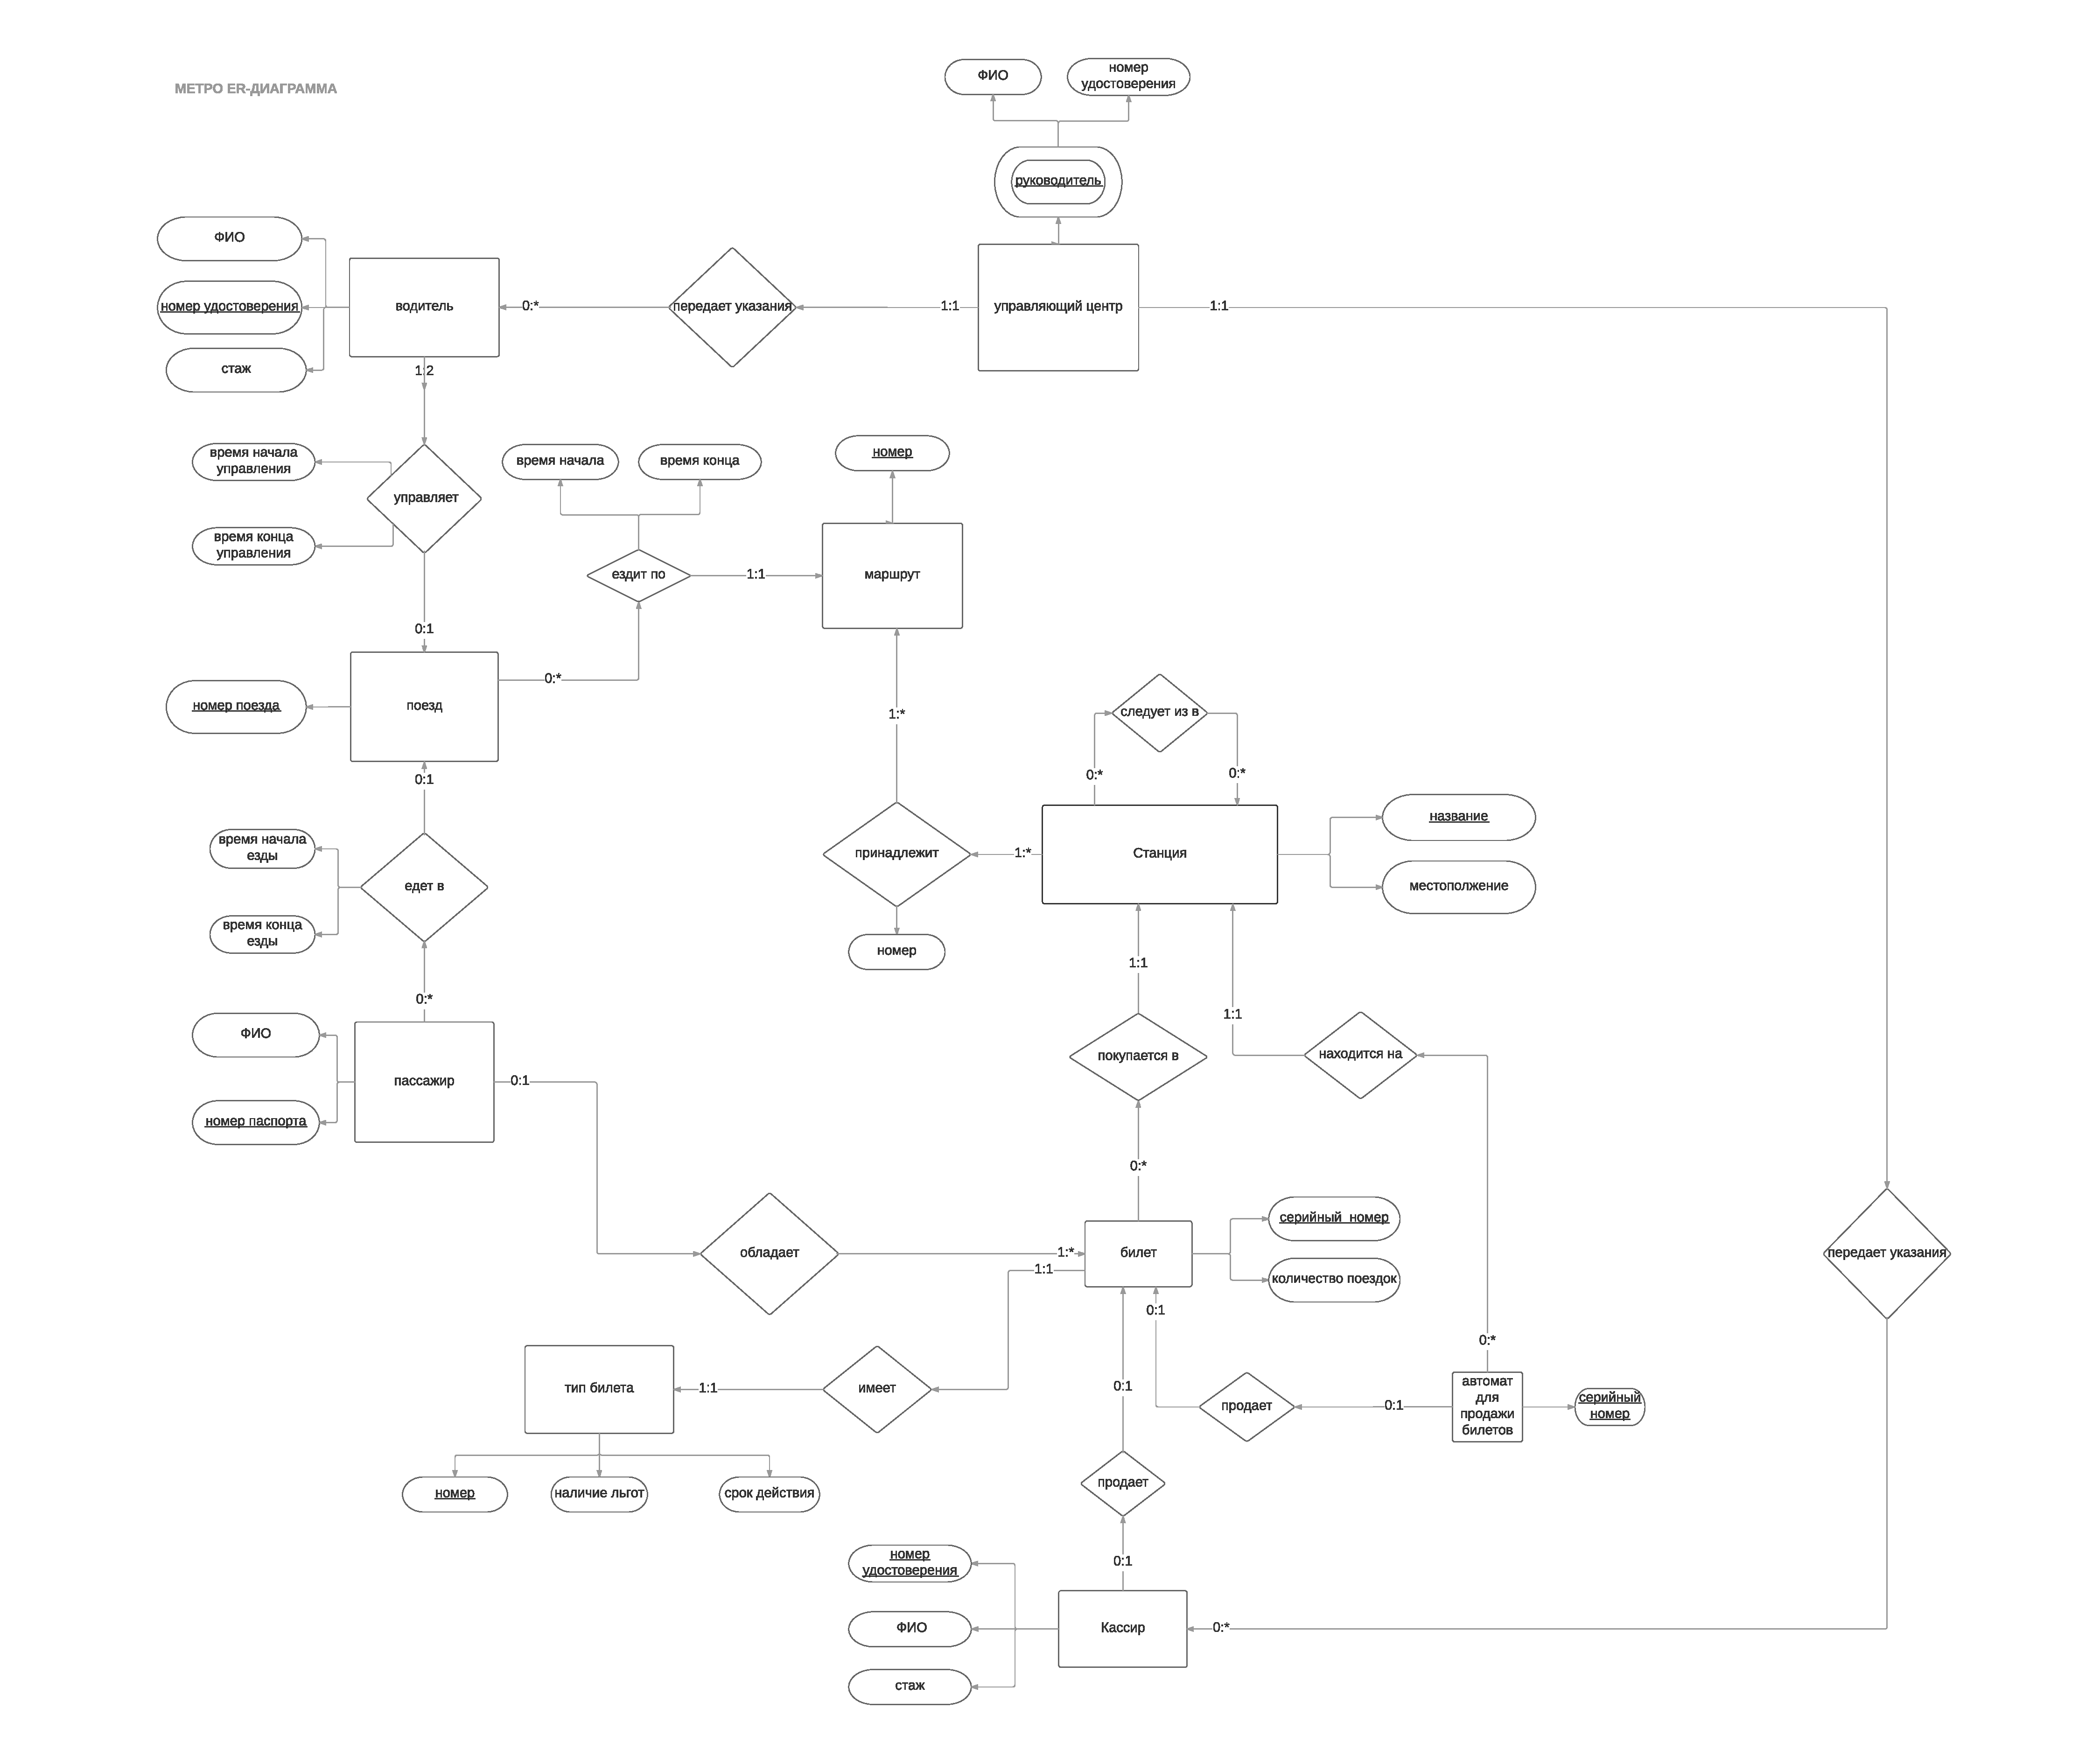
\includegraphics[width=1.15\textwidth]{Metro_model.pdf}
    \caption{ER-диаграмма}
    \label{fig:my_label}
\end{figure}
\newpage
\section{Реляционная модель}
\begin{table}[h!]
\centering
\begin{tabular}{|c|c|c|c|}
    \hline
    Имя поля & Тип поля & Содержание поля & Примечание \\
    \hline
    DriverID & Varchar(100) & номер удостоверения & первичный ключ \\
    Surname & Varchar(100) & фамилия & обязательное поле \\
    Name & Varchar(100) & имя & обязательное поле \\
    Patronymic & Varchar(100) & отчество & \\
    Experience & Integer & стаж & обязательное поле\\
    SessionBegining & Date & время начала управления & обязательное поле \\
    SessionEnd & Date & время конца управления & обязательное поле\\
    TrainID & Varchar(100) & номер поезда & внешний ключ (к Train)\\
    ManagerID & Varchar(100) & руководитель упр. центра & внешний ключ (к Manager) \\
    \hline
\end{tabular}
    \caption{Отношение <<Водитель>> (Driver)}
\end{table}

\begin{table}[h!]
\centering
\begin{tabular}{|c|c|c|c|}
    \hline
    Имя поля & Тип поля & Содержание поля & Примечание \\
    \hline
    TrainID & Varchar(100) & номер поезда & первичный ключ \\
    SessionBegining & Date & время начала & обязательное поле \\
    SessionEnd & Date & время начала & обязательное поле \\
    RouteID & Integer & номер маршрута & внешний ключ (к Route) \\
    \hline
\end{tabular}
    \caption{Отношение <<Поезд>> (Train)}
\end{table}

\begin{table}[h!]
\centering
\begin{tabular}{|c|c|c|c|}
    \hline
    Имя поля & Тип поля & Содержание поля & Примечание \\
    \hline
    RouteID & Varchar(100) & номер маршрута & первичный ключ \\
    \hline
\end{tabular}
    \caption{Сущность <<Маршрут>> (Route)}
\end{table}

\begin{table}[h!]
\centering
\begin{tabular}{|c|c|c|c|}
    \hline
    Имя поля & Тип поля & Содержание поля & Примечание \\
    \hline
    StationID & Varchar(100) & номер & первичный ключ \\
    StationName & Varchar(100) & название & обязательное поле \\
    \hline
\end{tabular}
    \caption{Сущность <<Станция>> (Station)}
\end{table}

\begin{table}[h!]
\centering
\begin{tabular}{|c|c|c|c|}
    \hline
    Имя поля & Тип поля & Содержание поля & Примечание \\
    \hline
    Id & Varchar(100) & номер & первичный ключ \\
    OrderNumber & Integer & порядковый номер & обязательное поле \\
    RouteID & Varchar(100) & номер маршрута & внешний ключ (к Route)  \\
    StationName & Varchar(100) & название станции & внешний ключ (к Station) \\
    \hline
\end{tabular}
    \caption{Отношение между маршрутом и станцией (RouteToStation)}
\end{table}

\begin{table}[h!]
\centering
\begin{tabular}{|c|c|c|c|}
    \hline
    Имя поля & Тип поля & Содержание поля & Примечание \\
    \hline
    Id & Varchar(100) & номер & первичный ключ \\
    StationName & Varchar(100) & название станции & внешний ключ (к Station) \\
    StationName & Varchar(100) & название станции & внешний ключ (к Station) \\
    \hline
\end{tabular}
    \caption{Отношение между станцией и станцией (StationToStation)}
\end{table}


\begin{table}[h!]
\centering
\begin{tabular}{|c|c|c|c|}
\hline
    Имя поля & Тип поля & Содержание поля & Примечание \\
    \hline
    Name & Varchar(100) & название & первичный ключ  \\
    Priveleges & Varchar(100) & льготы &  \\
    Termination & Date & день истечения срока действия & обязательное поле \\
    \hline
\end{tabular}
    \caption{Сущность <<Тип билета>> (TicketType)}
\end{table}

\begin{table}[h!]
\centering
\begin{tabular}{|c|c|c|c|}
\hline
    Имя поля & Тип поля & Содержание поля & Примечание \\
    \hline
    CashierID & Varchar(100) & номер удостоверения & первичный ключ  \\
    Surname & Varchar(100) & фамилия & обязательное поле \\
    Name & Varchar(100) & имя & обязательное поле \\
    Patronymic & Varchar(100) & отчество & \\
    Experience & Integer & стаж & обязательное поле \\
    ManagerID & Varchar(100) & руководитель упр. центра & внешний ключ (к Manager) \\
    \hline
\end{tabular}
    \caption{Отношение <<Кассир>> (Cashier)}
\end{table}

\begin{table}[h!]
\centering
\begin{tabular}{|c|c|c|c|}
\hline
    Имя поля & Тип поля & Содержание поля & Примечание \\
    \hline
    TicketID & Varchar(100) & номер билета & первичный ключ  \\
    NumberOfTrips & Integer & количество поездок & обязательное поле \\
    TypeOfTicket & Varchar(100) & тип билета & внешний ключ (к TicketType) \\
    PassengerID & Varchar(100) & пассажир & (необяз.) внешний ключ (к Passenger) \\
    StationName & Varchar(100) & имя станции & внешний ключ (к Station) \\
    CashierID & Varchar(100) & кассир & (необяз.) внешний ключ (к Cashier) \\
    MachineID & Varchar(100) & автомат & (необяз.) внешний ключ (к TicketMachine) \\
    \hline
\end{tabular}
    \caption{Отношение <<Билет>> (Ticket)}
\end{table}


\begin{table}[h!]
\centering
\begin{tabular}{|c|c|c|c|}
\hline
    Имя поля & Тип поля & Содержание поля & Примечание \\
    \hline
    PassengerID & Varchar(100) & номер паспорта & первичный ключ \\
    Surname & Varchar(100) & фамилия & обязательное поле \\
    Name & Varchar(100) & имя & обязательное поле \\
    Patronymic & Varchar(100) & отчество & \\
    TrainID & Varchar(100) & номер поезда & (необяз.) внешный ключ (Train) \\
    \hline
\end{tabular}
    \caption{Отношение <<Пассажир>> (Passenger)}
\end{table}

\begin{table}[h!]
\centering
\begin{tabular}{|c|c|c|c|}
\hline
    Имя поля & Тип поля & Содержание поля & Примечание \\
    \hline
    MachineID & Varchar(100) & номер автомата & первичный ключ \\
    StationName & Varchar(100) & имя станции &  (необяз.) внешный ключ (Station) \\
    TicketID & Varchar(100) & номер билета & внешный ключ (Ticket) \\
    \hline
\end{tabular}
    \caption{Отношение <<Автомат>> (TicketMachine)}
\end{table}

\begin{table}[h!]
\centering
\begin{tabular}{|c|c|c|c|}
\hline
    Имя поля & Тип поля & Содержание поля & Примечание \\
    \hline
    ManagerID & Varchar(100) & номер удостоверения & первичный ключ\\
    Surname & Varchar(100) & фамилия & обязательное поле \\
    Name & Varchar(100) & имя & обязательное поле \\
    Patronymic & Varchar(100) & отчество & \\
    \hline
\end{tabular}
    \caption{Сущность <<Руководитель управляющего центра>> (Manager)}
\end{table}
\newpage~
\section{Создание базы данных, запросы и приложение}
Создание базы данных, запросы и приложение было решено оформить с помощью Ipython Notebook-а. Ссылка: \url{https://nbviewer.jupyter.org/github/Ramil0/SQL/blob/master/metro_database.ipynb}


\section{Список литературы}
\begin{enumerate}
    \item Словарь <<Академика>>: \url{http://dic.academic.ru}
    \item Официальный сайт московского метрополитена: \url{http://mosmetro.ru/}
\end{enumerate}

\end{document} % конец документа